% This is samplepaper.tex, a sample chapter demonstrating the
% LLNCS macro package for Springer Computer Science proceedings;
% Version 2.20 of 2017/10/04
%
\documentclass[runningheads]{llncs}


%%%%%%%%%%%%%%%%%%%%%%%%%%%%%%%%%%%%%%%%%%%%%%%%%%%%%%%%%%%%%%%%%%%%
%% References                           						  %%
%%%%%%%%%%%%%%%%%%%%%%%%%%%%%%%%%%%%%%%%%%%%%%%%%%%%%%%%%%%%%%%%%%%%
\usepackage{hyperref}
\usepackage{cleveref}

%%%%%%%%%%%%%%%%%%%%%%%%%%%%%%%%%%%%%%%%%%%%%%%%%%%%%%%%%%%%%%%%%%%%
%% Acronyms                           							  %%
%%%%%%%%%%%%%%%%%%%%%%%%%%%%%%%%%%%%%%%%%%%%%%%%%%%%%%%%%%%%%%%%%%%%
\usepackage{acro}

\makeatletter
\@ifpackagelater{acro}{2017/02/17}{\@ifpackagelater{acro}{2019/09/23}{}{
	\let\IDeclareAcronym\DeclareAcronym
	\renewcommand{\DeclareAcronym}[2]{%
		\IDeclareAcronym{#1}{%
		#2,foreign-plural={}
		}
	}
}}{}
\makeatother

\newcommand\ifacrothree{%
	\ifnum\numexpr\csname c_acro_version_major_number_tl\endcsname=3\relax
}

\ifacrothree
	\acsetup{use-id-as-short}
	\def\ProvideAcroEnding{\DeclareAcroEnding}
\fi

\ProvideAcroEnding{possessive}{'s}{'s}
\ProvideAcroEnding{possessiveplural}{s'}{s'}

\ifacrothree
	\NewAcroCommand\acg{m}{%
		\acropossessive
		\UseAcroTemplate{first}{#1}%
	}
	\NewAcroCommand\acsg{m}{%
		\acropossessive
		\UseAcroTemplate{short}{#1}%
	}
	\NewAcroCommand\aclg{m}{%
		\acropossessive
		\UseAcroTemplate{long}{#1}%
	}
	\NewAcroCommand\acgp{m}{%
		\acropossessiveplural
		\UseAcroTemplate{first}{#1}%
	}
	\NewAcroCommand\acsgp{m}{%
		\acropossessiveplural
		\UseAcroTemplate{short}{#1}%
	}
	\NewAcroCommand\aclgp{m}{%
		\acropossessiveplural
		\UseAcroTemplate{long}{#1}%
	}
\else
	% remove this part when acro-2 (texlive-2019) is no longer in use by any sane person
	% e.g. ubuntu-20.04 has texlive-2019 and will receive updates until April 2025
	\ExplSyntaxOn
	\NewAcroCommand \acg {
		\acro_possessive:
		\acro_use:n {#1}
	}
	\NewAcroCommand \acsg {
		\acro_possessive:
		\acro_short:n {#1}
	}
	\NewAcroCommand \aclg {
		\acro_possessive:
		\acro_long:n {#1}
	}
	\NewAcroCommand \acgp {
		\acro_possessiveplural:
		\acro_use:n {#1}
	}
	\NewAcroCommand \acsgp {
		\acro_possessiveplural:
		\acro_short:n {#1}
	}
	\NewAcroCommand \aclgp {
		\acro_possessiveplural:
		\acro_long:n {#1}
	}
	\ExplSyntaxOff
\fi

% Common
\DeclareAcronym{DLR}{short=DLR, long=Deutsches Zentrum für Luft- und Raumfahrt (eng.: German Aerospace Center)}
\DeclareAcronym{SSH}{short=SSH, long=Secure Shell}

% Background
\DeclareAcronym{BDD}{short=BDD, long=Behaviour Driven Development}
\DeclareAcronym{DDD}{short=DDD, long=Domain-driven Design}
\DeclareAcronym{TDD}{short=TDD, long=Test-Driven Development}
\DeclareAcronym{DSL}{short=DSL, long=Domain-specific Language}
\DeclareAcronym{GUI}{short=GUI, long=Graphical User Interface}
\DeclareAcronym{Regex}{short=Regex, long=Regular Expression}

% RCE
\DeclareAcronym{RCE}{short=RCE, long=Remote Component Environment}
\DeclareAcronym{IM}{short=IM, long=Instance Management Component}
\DeclareAcronym{TSR}{short=TSR, long=Test Script Runner}

% Examination
\DeclareAcronym{JDK}{short=JDK, long=Java Development Kit}
\usepackage{booktabs}% http://ctan.org/pkg/booktabs

%%%%%%%%%%%%%%%%%%%%%%%%%%%%%%%%%%%%%%%%%%%%%%%%%%%%%%%%%%%%%%%%%%%%
%% Listings                           							  %%
%%%%%%%%%%%%%%%%%%%%%%%%%%%%%%%%%%%%%%%%%%%%%%%%%%%%%%%%%%%%%%%%%%%%
\crefname{lstlisting}{listing}{listings}
\Crefname{lstlisting}{Listing}{Listings}
\usepackage{graphicx}
\usepackage{xcolor}
\usepackage[newfloat]{minted}
\usepackage{listings}

% Used for displaying a sample figure. If possible, figure files should
% be included in EPS format.
%
% If you use the hyperref package, please uncomment the following line
% to display URLs in blue roman font according to Springer's eBook style:
\renewcommand\UrlFont{\color{blue}\rmfamily}

\begin{document}
%
\title{Analysis of BDD Testing in RCE: Enhancing Framework Resilience through Evaluation and Recommendations}
%
\titlerunning{Analysis of BDD Testing in RCE}
% If the paper title is too long for the running head, you can set
% an abbreviated paper title here
%
\author{Artur Komaristych\inst{1} \and Luka Gerlach\inst{1}}
%
\authorrunning{A. Komaristych, L. Gerlach}
% First names are abbreviated in the running head.
% If there are more than two authors, 'et al.' is used.
%
\institute{University of Cologne \and
DLR Institute for Software Technology}
%
\maketitle              % typeset the header of the contribution
%
\begin{abstract}
With the proliferation of distributed systems, robust testing methodologies have become paramount to ensure seamless integration and reliability. This paper examines the adoption of a \ac{BDD} Testing Approach by influential entities like the \ac{DLR} in their distributed application, the \ac{RCE}. A comprehensive analysis of RCE's BDD testing setup is presented, offering valuable insights into potential challenges encountered in testing distributed systems. Furthermore, the focus extends to an unexplored facet of network testing within RCE, specifically addressing the introduction of artificial network failures to simulate real-world complexities. This exploration aims to improve our understanding of the efficacy of BDD testing in the context of RCE and contribute to the broader discourse on testing methodologies for distributed systems.
%\keywords{First keyword  \and Second keyword \and Another keyword.}
\end{abstract}
%
%
%
\section{Introduction}
As the landscape of software development continues to evolve, the employment of distributed systems has become increasingly widespread.~\cite{Xingang2018,Feldman1978}. The paradigm shift from centralized towards distributed systems brings forth a new set of challenges, particularly in the realm of testing, as traditional methodologies often struggle to encapsulate the complexities inherent to these distributed architectures~\cite{Liu,Lima2017}. Testing distributed applications as holistic entities, rather than isolated components, has become a necessary practice to ensure seamless integration and robust functionality~\cite{Liu,Lima2017}.

Traditional testing methodologies, designed for monolithic systems, often fall short in capturing the intricate dependencies and interactions among distributed components~\cite{Liu,Lima2017}. This challenge becomes particularly apparent when considering the~\acf{RCE}, developed by the~\acf{DLR}. \ac{RCE}, as a distributed system, encapsulates the complexities inherent in network applications, demanding a departure from conventional testing norms.

Within \ac{RCE}'s server-based remote component architecture, client instances operate as thin clients, accessing server-provided components and functionalities within a complex calculation and simulation workflow. A \ac{RCE} workflow comprises components with predefined inputs and outputs connected to each other, thereby defining the data flow. This design emphasizes the need for a comprehensive testing approach, as unexpected behavior of remote server instances, coupled with network-shared components, could render the client application useless or lead to inaccurate calculations.

Unlike the conventional approach of testing individual components locally, \ac{RCE} employs a testing strategy aligned with real-world deployment scenarios, implementing a \acf{BDD} testing strategy. This \ac{BDD} methodology emphasizes the application's complete behavior and functionality from the user's point of view, guaranteeing that the system functions seamlessly and meets the expectations of the end user~\cite{wynne2012cucumber}. Using tools such as the \ac{DSL} Gherkin to formulate requirements in natural language (\Cref{subsec:gherkin}) and Cucumber to link these requirements to actual test cases (\Cref{subsec:cucumber}), this approach not only addresses the challenges of testing distributed applications, but also underscores the importance of a collaborative and holistic testing paradigm.

By extracting valuable insights about \ac{RCE}'s testing methodology and exploring ways to enhance it, this paper aims to provide actionable suggestions for strengthening the \ac{BDD} test setup in \ac{RCE}. We provide necessary background on fundamental concepts in~\Cref{sec:background} and our research methodology in~\Cref{sec:method}. We then examine the \ac{RCE} project and present our findings in~\Cref{sec:examination}, subsequently offering possible solutions in~\Cref{sec:results}. These solutions are evaluated in~\Cref{sec:discussion} and a brief summary of our work is given in~\Cref{sec:conclusion}.
\section{Background and Related Work}
\label{sec:background}
\subsection{\acl{BDD}}
\label{subsec:bdd}
\acf{BDD} is a software development practice intricately woven into the framework of agile methodologies, that frames system design and development around end user expectations about the system and how it behaves. It positions itself as a dynamic response to prevalent challenges by prioritizing the user perspective and aligning closely with business needs. Based on the integration of concepts from both \ac{TDD} and \ac{DDD}, \ac{BDD} transcends traditional development paradigms.

\ac{BDD} stands out as a departure from the typical \ac{TDD} methodology, where the primary focus is on writing tests for isolated code units, with a predominant technical viewpoint, that restricts the determination of system behavior to developers and does not consider the system altogether. Instead, \ac{BDD} broadens its perspective, bridging the gap between technical and business aspects~\cite{Farooq2023bdd,Binamungu2020bdd} and allowing the. It achieves this by incorporating viewpoints from both spheres, redirecting the evaluation from individual code segments to the holistic assessment of the application's behavior from the user's standpoint. This strategic change not only enhances communication, but also fosters collaboration between developers, testers, and business stakeholders, as evidenced by previous research~\cite{smart2023bdd,pereira2018behavior}.

Rooted in a user-centric philosophy, test cases are structured using a language that mirrors natural language, thus enabling non-technical stakeholders to define system behavior and overcoming the challenge of system design being solely within the realm of developers, not seen as a whole. This approach serves as a catalyst for effective collaboration, creating a shared understanding among team members throughout the software development lifecycle.

\subsection{Gherkin}
\label{subsec:gherkin}

Gherkin is a \ac{DSL} prominently utilized in the domain of \ac{BDD}. It is used to create requirements and tests in a clear and human-readable format. Gherkin's syntax follows a systematic Given-When-Then structure, interweaving natural language expressions, as demonstrated in \Cref{lst:withdrawcash}. Therefore, it focuses on the end-user's perspective and business requirements rather than the underlying technical implementation.

\begin{listing}[!ht]
\caption{Exemplary feature file with one scenario. Adapted from 
\href{https://cucumber.io/blog/bdd/getting-started-with-bdd-part-1/}{cucumber.io}~\cite{noauthor_getting_nodate}}.
\label{lst:withdrawcash}
\inputminted{gherkin}{files/code/atm.feature}
\end{listing}

 Gherkin employs a distinct set of keywords to delineate various aspects of test scenarios. In particular, it utilizes the \texttt{feature} keyword to expound upon the primary functionality of the feature under examination, \texttt{Scenario} to specify individual use cases within the feature, \texttt{Given}-steps to establish initial context or preconditions, \texttt{When}-steps for denoting the event or action that triggers the scenario, and \texttt{Then}-steps for articulating anticipated outcomes for validation\footnote{It is imperative to acknowledge that this chapter does not exhaustively cover all Gherkin keywords, but rather focuses on those pertinent to our study. A comprehensive list is available at \href{https://cucumber.io/docs/gherkin/reference/\#keywords}{https://cucumber.io/docs/gherkin/reference}}. Furthermore, the \texttt{And} keyword facilitates the chaining of multiple steps of the same type, ensuring a logically granular and encapsulated representation of test steps. 
 
 This structural arrangement cultivates a shared understanding among stakeholders about the expected behavior of the system, thereby mitigating the previously defined structural challenges. In particular, this structure aligns well with user stories and other agile methodologies, providing a sufficient structure for interpretation by frameworks such as Cucumber to map individual test steps to executable code~\cite{noauthor_gherkin_nodate}.


\subsection{Cucumber}
\label{subsec:cucumber}
Cucumber\footnote{https://cucumber.io/} is an open-source software primarily utilized for conducting \ac{BDD} tests. The Cucumber Open platform offers libraries for various programming languages, such as Java, JavaScript, Ruby, .NET, and others, providing all the essential functionality needed for parsing Gherkin files~\cite{noauthor_cucumber_nodate}. These libraries enable the mapping of natural language descriptions of software requirements, found in Gherkin files, to specific test implementation steps. This comprehensive functionality facilitates the execution of Gherkin-based automated tests, effectively linking natural language descriptions to executable code.~\cite{wynne2012cucumber}.

\begin{figure}
    \centering
    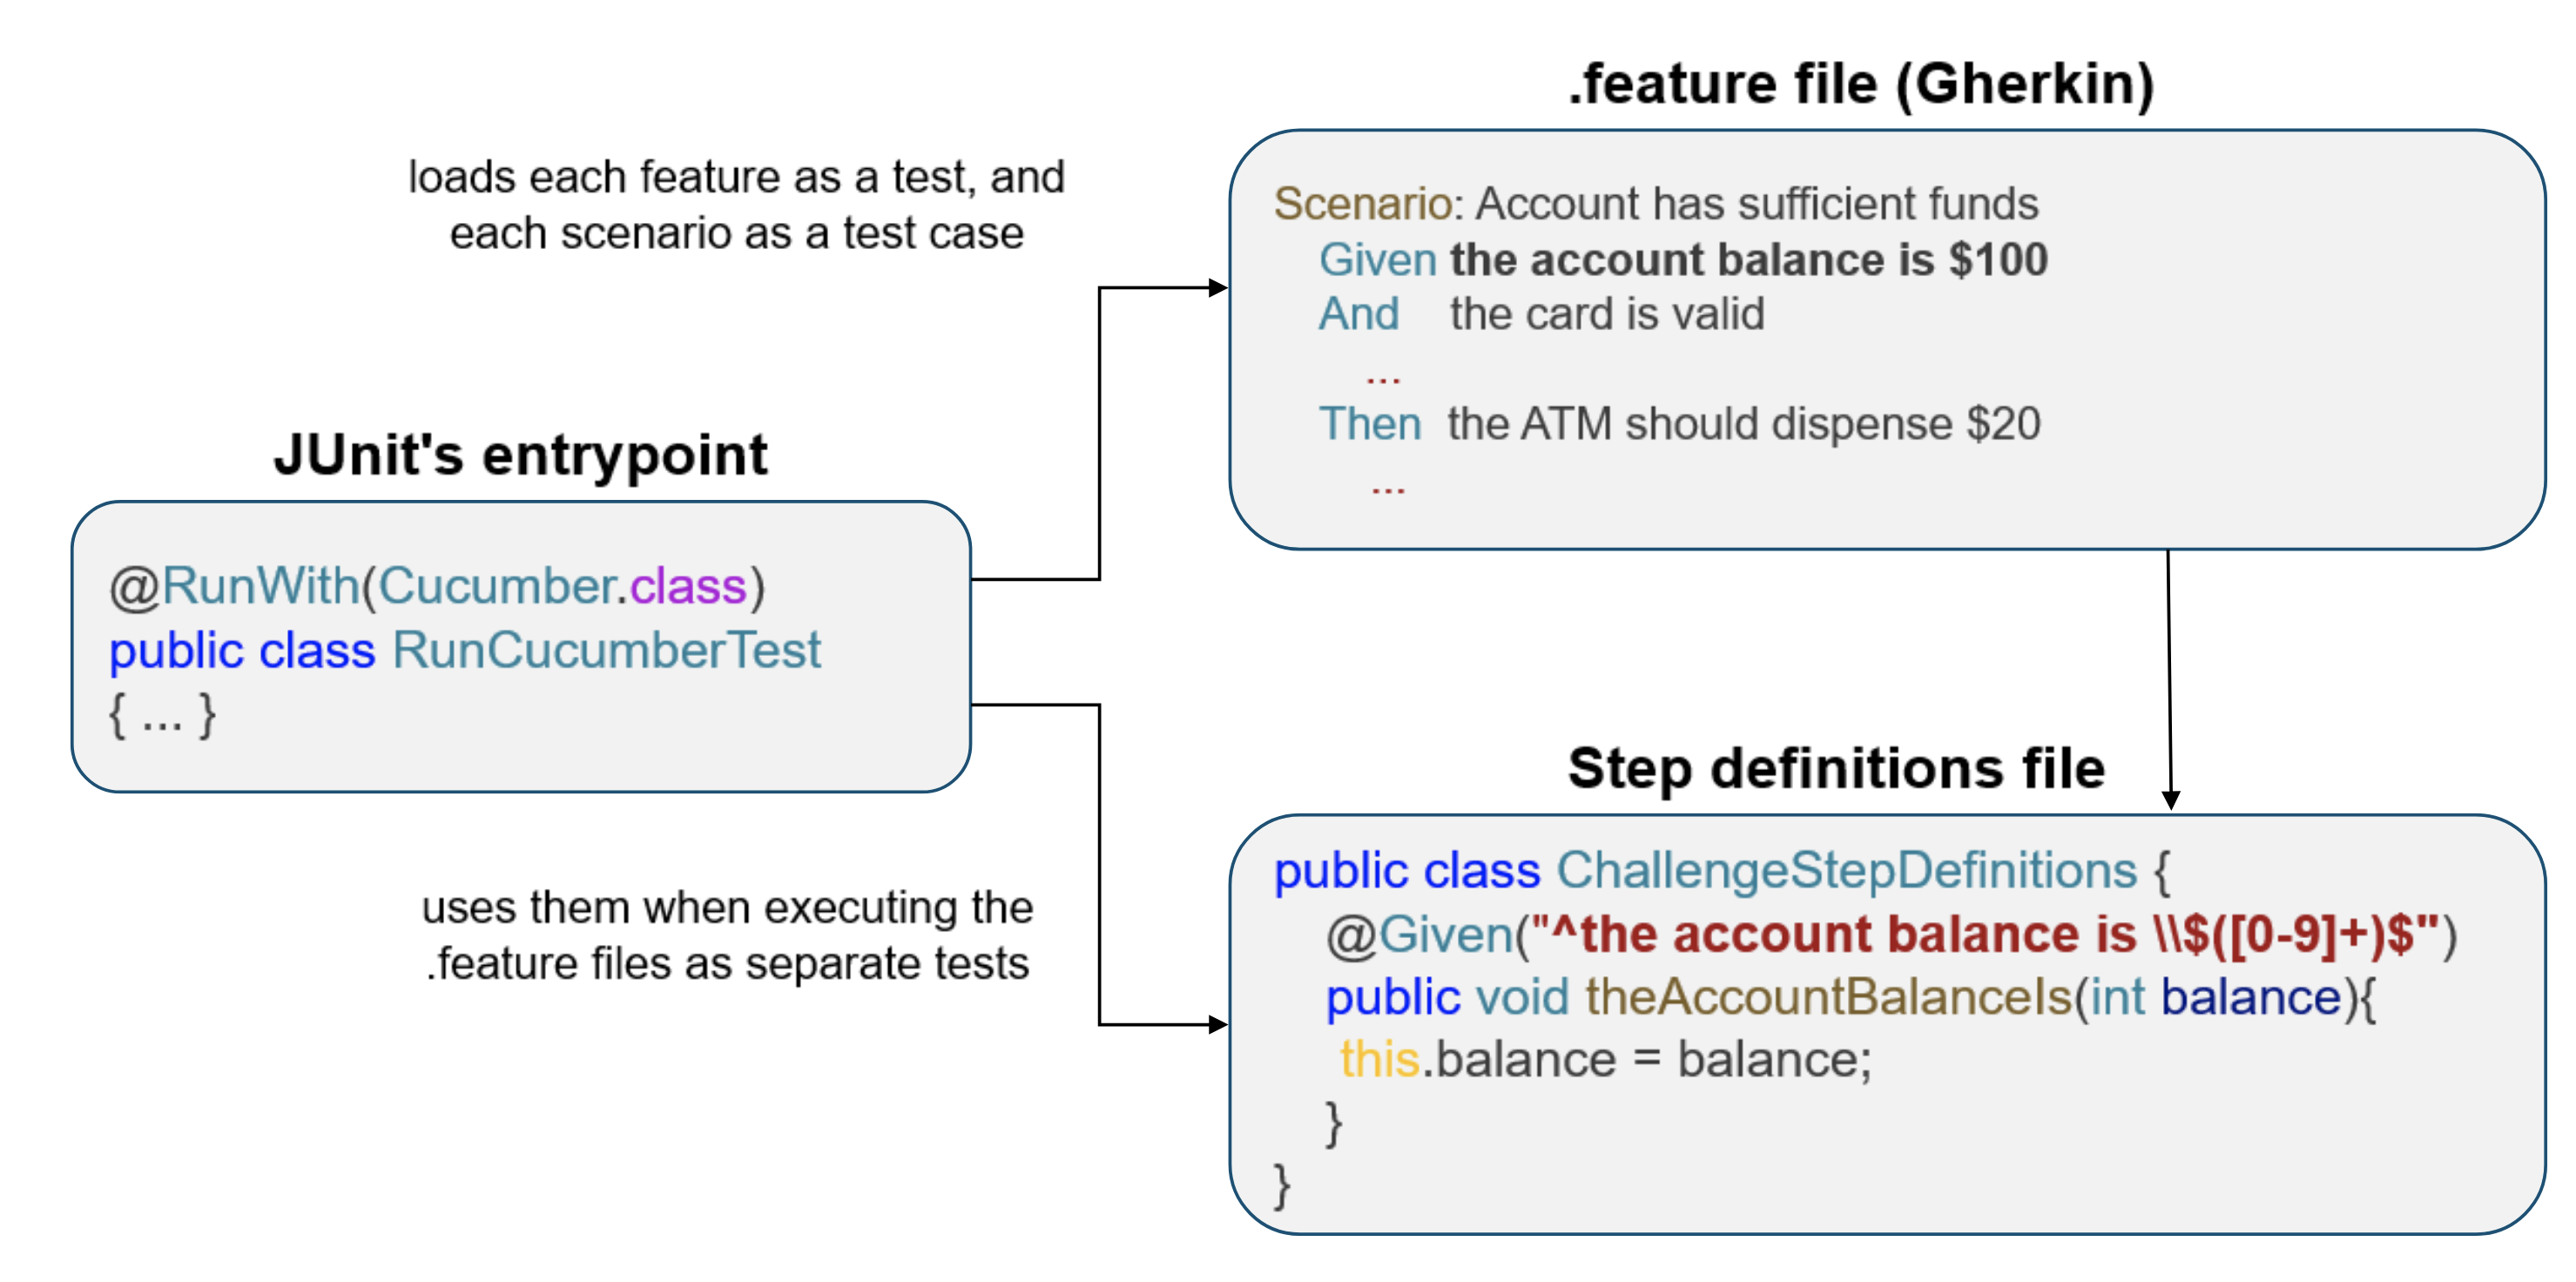
\includegraphics[width=\linewidth]{files/figures/cucumber_test_step_mapping.png}
    \caption{Illustration how Cucumber is used to link natural language clauses and their respective Java implementations}
    \label{fig:cucumber-mapping}
\end{figure}

Based on the scenario described in~\Cref{lst:withdrawcash}, the corresponding~\Cref{fig:cucumber-mapping} illustrates the connection between the specified natural language test steps and their concrete code representations. In the context of Java, developers use annotations to specify Java methods as implementations of steps in a Gherkin file. These annotations incorporate a regex string, and when a sentence in a Gherkin step matches this string, it triggers the execution of the corresponding Java method. For instance, the \texttt{theAccountBalanceIs} function, annotated with \texttt{@Given} and featuring a regex pattern, is invoked when the regex matches a sentence in a ``GIVEN`` clause, e.g., ``the account balance is \$100``~\cite{noauthor_bdd_nodate}.

\subsection{Distributed Systems}
\label{subsec:dissys}
A distributed system is a network of independent computers, running on multiple servers or nodes, that interact and synchronize their activities through the exchange of information~\cite{tanenbaum2007distributed}. These systems consist of components that collaboratively work towards a shared objective, presenting advantages in terms of performance, scalability, and redundancy when compared to centralized systems. The shift from centralized architectures towards distributed systems is motivated by the inadequacies of non-distributed, centralized computing models, typified by a single monolithic server. Such centralized models have proven insufficient in addressing the increasing computational requirements and the need for enhanced system capabilities that could not be mitigated by vertically scaling a single system.

The distinctive feature of distributed systems lies in their avoidance of shared computing and memory resources, introducing complexities related to heterogeneity, scalability, and failure handling, among other challenges~\cite{coulouris2005distributed}. Non-distributed systems may struggle to effectively manage these challenges, leading to limitations in performance, scalability, and fault tolerance. Distributed systems, by distributing computational tasks across a network of interconnected computers, address these shortcomings~\cite{coulouris2005distributed}.

For instance, consider a scenario where a centralized system, operating on a single powerful server, reaches the maximum capacity of available hardware resources. Upgrading the hardware of that single machine (vertically scaling), may become impractical or cost-prohibitive. In such situations, distributed systems offer a viable solution. By distributing the workload across multiple interconnected nodes, these systems enable parallel processing, allowing for efficient utilization of available resources beyond the constraints of a single machine. 

However, this comes at the cost of complexity, as these clusters of individual computers need to be carefully coordinated and managed. Additionally, information must be transferred from one host to another, introducing non-determinism, particularly through the network, as a source of unpredictability. This introduces the potential for errors, such as when packages are lost during the communication between nodes.

\subsection{\acl{RCE}}
\label{subsec:rce}
\ac{RCE}\footnote{https://rcenvironment.de/} is an open-source application primarily developed at the \ac{DLR}. It is designed to facilitate the multidisciplinary engineering process, especially in complex system engineering such as aerospace, allowing users to integrate various disciplinary tools, define their dependencies, and execute multidisciplinary workflows~\cite{BODEN2021100759}. A key feature of \ac{RCE} is its ability to connect different \ac{RCE} instances in a distributed system, which greatly facilitates collaboration between various departments and specializations. This interconnected approach allows engineers from multiple disciplines to contribute their individual tools to a unified workflow, enhancing efficiency and reducing the propensity for errors in complex engineering projects. In this paper, our focus will be limited to those aspects of \ac{RCE} that are relevant to our project. Consequently, many features and advantages of \ac{RCE} that extend beyond the scope of our work will not be addressed here. For a comprehensive presentation of \ac{RCE} as well as its capacity to facilitate multidisciplinary collaboration, the reader is directed to consult the detailed tool papers provided in \cite{BODEN2021100759,boden2019distributed}, which offer a wide range of insights into the broader applications and benefits of \ac{RCE}.~\cite{BODEN2021100759}

\subsection{Kubernetes}
\label{subsec:kubernetes}
\acf{K8S}\footnote{https://kubernetes.io/} is an open source container orchestration platform that has emerged as the cornerstone of contemporary cloud native application development. Originally crafted by Google and presently overseen by the \ac{CNCF}, \ac{K8S} serves as a versatile and powerful solution for automating the deployment, scaling, and administration of containerized applications~\cite{burns2022kubernetes}. Its architectural design facilitates the abstraction of infrastructure intricacies, providing developers with a standardized environment for the efficient deployment and management of microservices.~\cite{noauthor_production-grade_nodate}

\subsection{WinDivert}
\label{subsec:windivert}
WinDivert\footnote{https://github.com/basil00/Divert} is a dynamic and versatile open-source library designed specifically for Windows operating systems. Developed by Basil Hussain, it provides a user-mode packet capture-and-divert framework, enabling the interception, modification, and dropping of network packets.

\begin{figure}
    \centering
    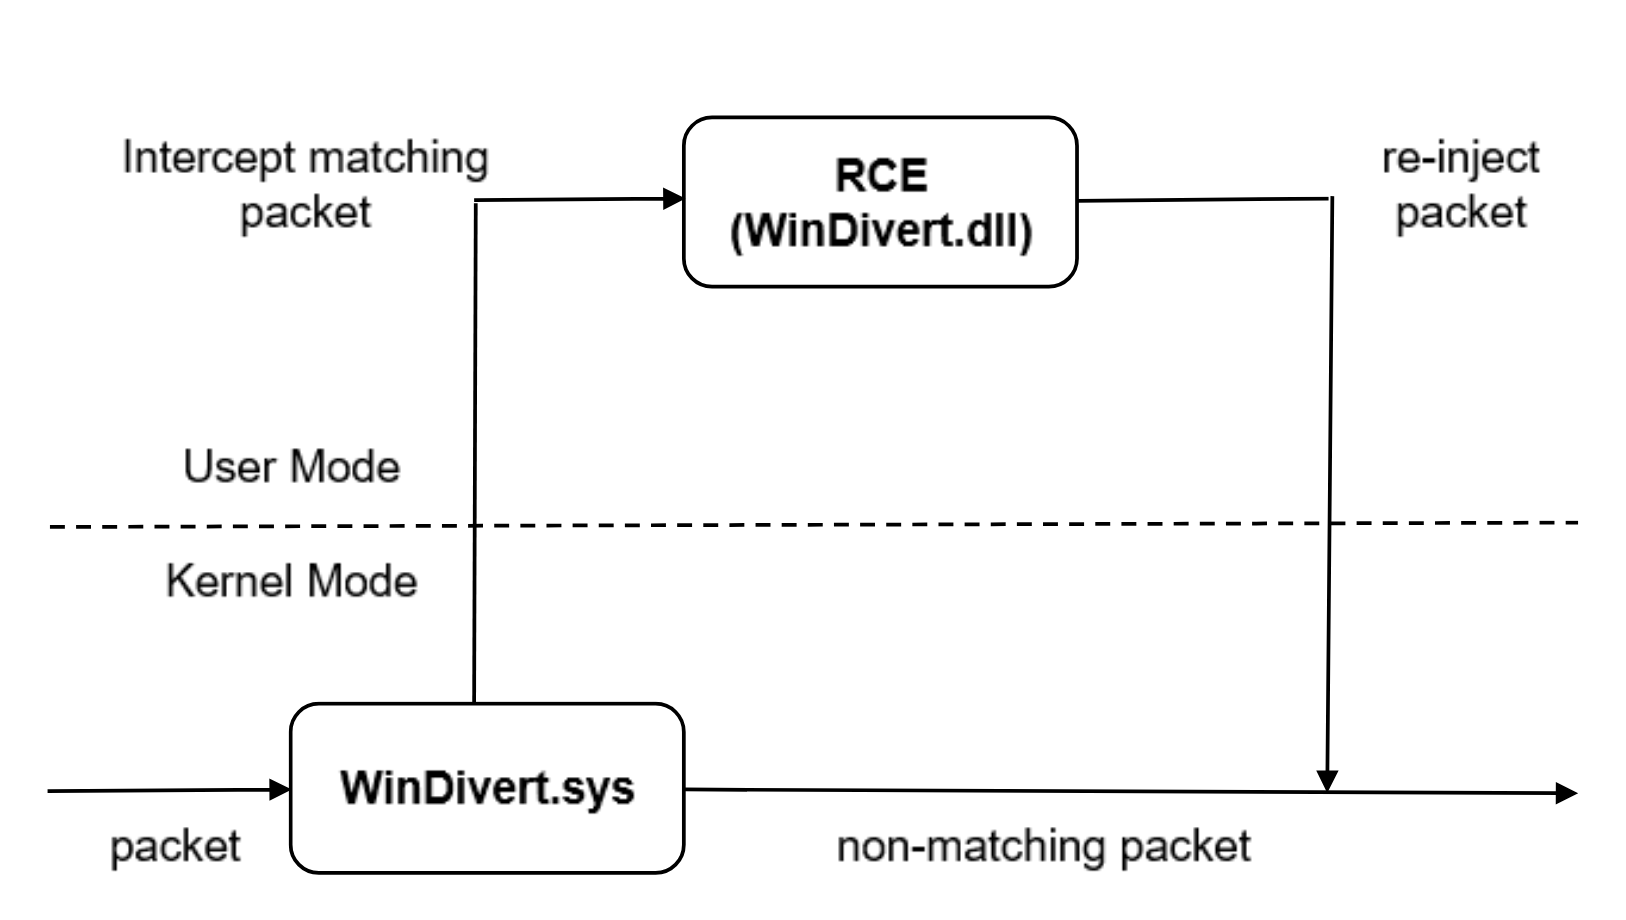
\includegraphics[width=\linewidth]{files/figures/WinDivert.png}
    \caption{WinDivert Architecture}
    \label{fig:WinDivert}
\end{figure}

As illustrated in ~\Cref{fig:WinDivert}, WinDivert operates at the kernel level, but can be incorporated on user level, allowing applications to exert fine-grained control over network traffic on Windows platforms. This library is particularly useful for implementing network-related functionalities, such as firewall applications, intrusion detection systems, and network testing tools. With its Java bindings, WinDivert can be seamlessly integrated into Java applications, making it an appealing choice for scenarios where precise control over network traffic is essential.~\cite{noauthor_windivert:_nodate}

\subsection{Chaos Mesh}
\label{subsec:chaosmesh}
Chaos Mesh is an open-source chaos engineering platform that facilitates the systematic testing and identification of weaknesses in distributed systems. Developed by the Chaos Mesh community, it provides a versatile set of tools for inducing chaos experiments within~\Cref{subsec:kubernetes} environments. These experiments aim to simulate real-world system failures and assess how well the system can withstand unexpected disruptions.

Chaos Mesh offers features such as fault injection, resource consumption testing, and network chaos, allowing users to replicate scenarios such as network delays, packet loss, and more. By orchestrating controlled chaos experiments, Chaos Mesh helps teams proactively discover and address potential vulnerabilities, leading to enhanced system resilience and reliability.~\cite{noauthor_chaos_nodate}
\section{Method}
\label{sec:method}
In this chapter, we introduce our task and discuss our chosen approach. First, in~\Cref{subsec:Task}, we describe the assignment. Subsequently, in~\Cref{subsec:Methodologies} we discuss the methods we selected to fulfill this assignment.

\subsection{Task Background}
\label{subsec:Task}
In the initial stages, our assignment was explicitly outlined and consists of the following tasks: 
\begin{enumerate}
    \item[A)] Compile the \ac{RCE}'s source code
    \item[B)] Review and execute the current tests in the \ac{RCE}. This examination seeks to comprehend the present testing framework employed, with the intention of subsequently offering valuable insights through a methodical evaluation.
    \item[B)] Examine the code base of the \acl{TSR} and Gherkin feature files to identify errors or areas that could be improved.
    \item[C)] Integrate enhancements into the existing codebase, focusing specifically on expanding network tests to assess the application's behavior in scenarios where the connection between two nodes is lost.
\end{enumerate}

\subsection{Methodology}
\label{subsec:Methodologies}
Based on the fact that our task could be divided into three subtasks, each pursuing a different objective, we have decided to employ various methods. Therefore, we decided to initially examine and extract information from the existing code to understand and trace the test structure in \ac{RCE} via an initial examination and documentation study.

Given the understanding of the respective technologies, we have decided to conduct an in-depth examination of the existing tests through a code review, coupled with the execution of the current test cases as a black box. This approach has the advantage that, firstly, by simply running the tests, we may discover test cases that yield negative results and point us to broken tests. Recognizing that the accuracy of test outputs is only as reliable as the tests themselves, we have opted to simultaneously perform a code review. This allows us to verify whether the tests are indeed evaluating what they purport to test. 

To address the last point on our agenda, which comprises implementing improvements and introducing new test cases, we have devised a strategy informed by the fact that we are not experts in the domain of \ac{RCE}. Given our limited familiarity with the software, we recognize the importance of adopting an exploratory approach to programming. This methodology proves advantageous in situations where comprehensive domain knowledge is lacking. By participating in exploratory programming, a process where developers iteratively experiment with the software, the goal is to uncover potential scenarios and functionalities that may not be immediately apparent through conventional testing methods. 

Exploratory programming involves an interactive and hands-on approach to better understand the software's behavior and discover aspects that may not have been initially considered during the development process. This approach allows us to supplement the existing testing framework with additional test cases, thus enhancing its robustness and expanding its coverage.
\section{Examination of the RCE Testing Setup}
\label{sec:examination}
In our investigation of the existing BDD testing setup in \ac{RCE}, we have organized the examination into several distinct subsections. The initial~\Cref{subsec:BuildingRCE} will focus on the practical steps associated with compiling \ac{RCE}, highlighting the procedures and challenges encountered during the successful compilation process. Subsequently, in~\Cref{subsec:PreparingRCETests}, we will elaborate on the configuration requirements for \ac{RCE} to enable the execution of the built-in test suite. Furthermore,~\Cref{subsec:BuiltinBDDTest} will focus on our examination of the BDD Testing Setup, the tests themselves, and our findings after applying a black-box testing paradigm. The fault tolerance of the built-in tests is then explored in~\Cref{subsec:fault-tolerance}.

Finally, transitioning to~\Cref{subsec:CodeReview}, we will undertake a more comprehensive code review of the actual source code. This thorough analysis involves examining how Cucumber is integrated within the codebase. We will unravel the complexities of the Gherkin \texttt{.feature} files and their interconnection with the corresponding Step Definition Code. This in-depth exploration is designed to illuminate the construction and execution of testing scenarios within \ac{RCE}'s application.

\subsection{Compiling \ac{RCE} from Scratch}
\label{subsec:BuildingRCE}
Initiating the compilation of \ac{RCE} involves a multistep process fully outlined in the \href{https://rcenvironment.de/pages/documentation/documentation.html}{RCE Developer Guide}~\cite{rceDevGuide10x}. The procedure includes downloading Eclipse IDE for RCP and RAP Developers and modifying \texttt{eclipse.ini} file to augment the Java heap size—a crucial adjustment aimed at alleviating potential memory overflow issues throughout the compilation process~\cite{rceDevGuide10x}.

Subsequently, the source-code must be obtained and imported into Eclipse. Multiple sources are available for obtaining the source code of \ac{RCE}, including the official RCE website. However, we chose to use the GitHub repository (\href{https://github.com/rcenvironment/rce-main}{RCE-Main GitHub Repository}) for several advantages. Choosing the GitHub repository allows us to access the code as a git repository rather than plain files, providing enhanced version control and collaboration capabilities. This decision aligns with modern development practices and facilitates a more seamless integration of the code into our development environment. Before importing the project into Eclipse, the guide states that the generation of OSGI bindings must first be enabled. Generation of \texttt{OSGI-INF} can be enabled by navigating to the Eclipse preferences (\texttt{ Window Preferences}), accessing the \texttt{ DS Plugin Development DS Annotations} page, and enabling the option to \texttt{Generate descriptors for annotated sources}. Additionally, the output directory must be set to \texttt{OSGI-INF/generated}~\cite{rceDevGuide10x}.

Once these steps are completed, the source code can be imported into Eclipse by adding it as an existing project. Following the import, the target platform must be set, a critical step to supply external artifacts, such as the Eclipse RCP framework and various libraries, must be set\footnote{Note: There is currently a discrepancy between the location of the repository specified in the target files of the RCE GitHub repositories (\href{https://github.com/rcenvironment/rce/blob/master/de.rcenvironment/eclipse/tp/remote/default_release_or_snapshot.target}{rce} and \href{https://github.com/rcenvironment/rce-main/blob/main/de.rcenvironment/eclipse/tp/remote/default_release_or_snapshot.target}{rce-main}) and the location of the repository referenced in the developer guide.}. For convenience, the guide recommends using the default target platform named \texttt{default\_release\_or\_snapshot.target}, located under \texttt{de.rcenvironment/eclipse/tp/remote} within the code base, by default~\cite{rceDevGuide10x}.

Following these steps as described in the guide, a successful compilation of \ac{RCE} was achieved. However, during the process on Linux, we encountered a specific issue, which, fortunately, was already documented in the developer guide. This issue required us to disable Windows-specific subprojects in the workspace for seamless compilation~\cite{rceDevGuide10x}. It is crucial to mention that using Eclipse IDE for RCP and RAP Developers is essential, as attempting to compile it on a regular Eclipse IDE for Java and DSL Developers proved unsuccessful. Still, we can confirm that the latest Eclipse RCP Version 2023-12 also yielded positive compilation outcomes.

\subsection{Preparing and executing \ac{RCE}'s BDD Tests}
\label{subsec:PreparingRCETests}
In the process of compiling and launching \ac{RCE} successfully, we then proceeded to execute the built-in BDD tests. Contrary to expectations, these tests are not executed separately through Eclipse or similar platforms; instead, they are integrated into the \ac{RCE} application itself as console commands and are included in every build by default. This decision may initially seem confounding, as this functionality is typically not of interest to regular users, but is more geared towards developers or system administrators. Furthermore, the incorporation of such functionality results in an expansion of the overall size of the \ac{RCE} bundle, even when it is not essential. 

However, including the test suite in all releases and making it easily available as console commands has the advantage that when the software does not work correctly, users can run the tests on their machines without additional setup steps. The test output can then be attached when submitting issues, aiding developers in debugging the problem.

The command in~\Cref{lst:run-tests-command} requires two arguments. Firstly, the tests to be executed, and secondly, the version of \ac{RCE} on which the tests should be performed. For example, the example command \texttt{run-test :all releases/10.5.0} results in the execution of the entire test suite, indicated by \texttt{:all}, on the \ac{RCE} release version \texttt{10.5.0}.

\begin{listing}[ht]
\caption{run-test command signature}
\label{lst:run-tests-command}
\begin{minted}{shell}
run-test[s] [--format pretty|json] 
    <comma-separated list of test ids> |--all
    <build id>
\end{minted}
\end{listing}

During the initial execution of the command, it becomes clear that a freshly bootstrapped \ac{RCE} instance is unable to execute the test suite; instead, it prompts an error message. This issue is associated with the necessary configuration of the \ac{IM} as a prerequisite for the test suite. Consequently, the \ac{IM} must be configured through \ac{RCE}'s configuration file. There, the \texttt{instanceManagement} configuration block must be added. This block defines the root directory where work files and managed RCE test installations will be stored. An illustrative example configuration is provided in~\Cref{lst:configuration-json}.

\begin{listing}[!ht]
\caption{InstanceManagement block entry in \ac{RCE}'s configuration.json}
\label{lst:configuration-json}
\inputminted[linenos, xleftmargin=2em]{json}{files/code/configuration.json}
\end{listing}

Upon adjusting the \ac{IM} config block and then reissuing the test command, the tests are executed as intended. Throughout this process, crucial information, such as the test status and potential errors, is presented in the console. This output is depicted in~\Cref{fig:rce-test-output}. The result is the successful completion of all tests without errors, suggesting, at least on the surface, the accurate processing of the tests by the application.

\begin{figure}[!ht]
    \centering
    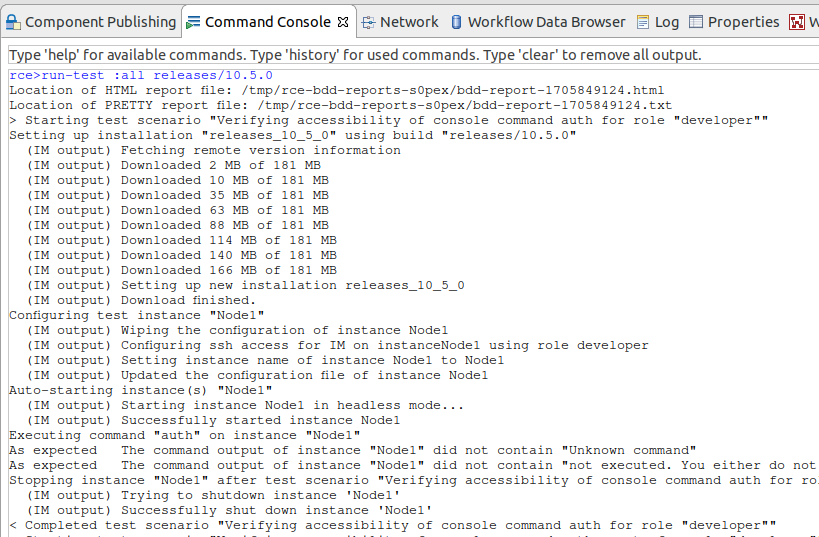
\includegraphics[width=\linewidth]{files/figures/rce-execute-tests.png}
    \caption{Example console output for command: \texttt{run-test :all releases/10.5.0}}
    \label{fig:rce-test-output}
\end{figure}


Although in this step we conducted only a very superficial black-box test through the execution of the tests, we were able to observe two noteworthy aspects. First, the \ac{RCE} tests encompass a diverse range of test cases, covering both functional tests (component, network communication, remote access, etc.) and the \ac{GUI} functionalities. Exclusively in \ac{GUI} tests, \ac{RCE} is launched with an authentic \ac{GUI}, and the functionalities are explicitly emulated through simulated clicks within the \ac{GUI}.
Executing the non-\acs{GUI}-based tests serves as a valuable test case, demonstrating that the typically \acs{GUI} based application can operate successfully without a \acs{GUI}. This testifies that the application can run on a server in a real-world scenario, i.e., without a display server. Additionally, it opens up the possibility of integrating these tests into a CI/CD pipeline, which often lacks the aforementioned display server.

Second, it became apparent that \ac{TSR} relies on \ac{IM} to start multiple \ac{RCE} instances configured as servers or clients. Therefore, we propose that the logic required to simulate a distributed environment is based heavily on the implementation of the \ac{IM} suggesting that it should be further analyzed in a subsequent step.

\subsection{\ac{RCE}'s BDD Testing Setup}
\label{subsec:BuiltinBDDTest}
In this subsection, we illuminate the workings of test execution. Initially, we provide a detailed overview of the setup and execution flow. Following that, we delve into how \ac{RCE} establishes a distributed system comprising multiple \ac{RCE} clients and servers locally. Next, we explain how \ac{RCE} overcomes the challenge of triggering behaviors and obtaining the state to properly evaluate the test cases across multiple clients and servers correctly. Finally, we offer a brief summary and conclusion.

\subsubsection{\ac{RCE}'s Test Setup and Execution Details in RCE}
The specifics of the Test Setup are detailed in \ac{RCE}'s Developer Guide~\cite{rceDevGuide10x} and thoroughly discussed in the work by Mischke et al. (2022)~\cite{10.1007/978-3-031-08760-8_44}. In essence, the test setup for \ac{RCE} revolves around the implementation of its test suite through a specialized component, called \acf{TSR}. This component assumes the responsibility of interpreting Gherkin files and executing tests under predefined conditions. To process Gherkin files, \ac{TSR} leverages the Cucumber library~\cite{10.1007/978-3-031-08760-8_44}, facilitating the mapping of free expressions in Gherkin to the corresponding actions executed during tests.

Within Gherkin feature files, the ``GIVEN`` clauses stipulate, for example, that \ac{TSR} must instantiate multiple client and server instances of \ac{RCE}. This initiation is facilitated by delegating the launch of numerous \ac{RCE} instances via the \acf{IM}~\cite{rceDevGuide10x}. 
The \ac{IM} plays a crucial role in overseeing \ac{RCE} instances used for testing purposes, which includes tasks such as downloading \ac{RCE}, initiating, and terminating instances~\cite{10.1007/978-3-031-08760-8_44,rceDevGuide10x}. Given that the tests can be instantiated even in a localized environment without a network connection, emphasizing the self-sufficiency of the testing process and providing flexibility in conducting tests in isolated settings without external dependencies, the need for \ac{IM} to instantiate the required instances locally becomes apparent.

This assumption can be easily verified using tools such as Task Manager, Process Hacker, htop, etc. Upon monitoring of the processes running during the tests, it becomes apparent that individual \ac{RCE} instances are instantiated as subprocesses of the primary \ac{RCE} instance. This observation aligns with the test description provided by Mischke et al. (2022)~\cite{10.1007/978-3-031-08760-8_44}. This strategic approach enables \ac{RCE} to emulate a locally distributed system with multiple independent instances, facilitating the testing of the implementation of network communication on the loopback device (i.e.,\texttt{localhost}). Consequently, the necessity of establishing and configuring a distributed system across multiple nodes can be mitigated. However, it is essential to acknowledge that this methodology has inherent limitations, as expounded on~\Cref{sec:results}.

In this context, an inquiry arises regarding the monitoring of autonomous processes by the \ac{TSR} and the subsequent execution of actions on them. Specifically, how does the \ac{TSR} handle the absence of direct access to instances instantiated by itself? This limitation presents a challenge in retrieving the state of these instances for the execution of Gherkin ``THEN`` clauses. Additionally, addressing the need for a mechanism to remotely perform actions on the launched RCE instances becomes imperative for the execution of ``WHEN`` clauses.

\subsubsection{Monitoring and Executing Actions on autonomous RCE instances}
As outlined, individual RCE instances are instantiated as autonomous processes. The encapsulation of these processes, which prohibits direct interaction, necessitates an alternative channel for interaction. Specifically, there must be a mechanism through which the \ac{TSR} can instruct individual instances to establish connections and execute workflows or analogous operations. Furthermore, it is crucial to validate the execution of workflows or the establishment of connections between instances. Given that these processes ideally operate independently within a distributed system, these operations must be performed through network communication.

Examination of the \ac{RCE} Developer and Admin Guide reveals various Command Console commands that offer the required functionality for executing necessary actions and retrieving relevant information~\cite{rceDevGuide10x}. Additionally, instances can be configured for accessibility via \ac{SSH}, enabling the remote execution of commands—without requiring physical access to the machine running RCE~\cite{rceDevGuide10x}. \ac{SSH} operates as a secure, text-based console, allowing encrypted remote communication and device management over unsecured networks. Hence, executing the aforementioned console commands over \ac{SSH} is crucial, especially when \ac{RCE} functions as a service, running the process in the background (i.e., without \texttt{--console}), thereby avoiding the display of the Command Console. In theory, this \ac{SSH} setup could also be used to address the challenge of accessing the state or executing operations in autonomous \ac{RCE} instances during local tests.

\begin{figure}[h]
    \centering
    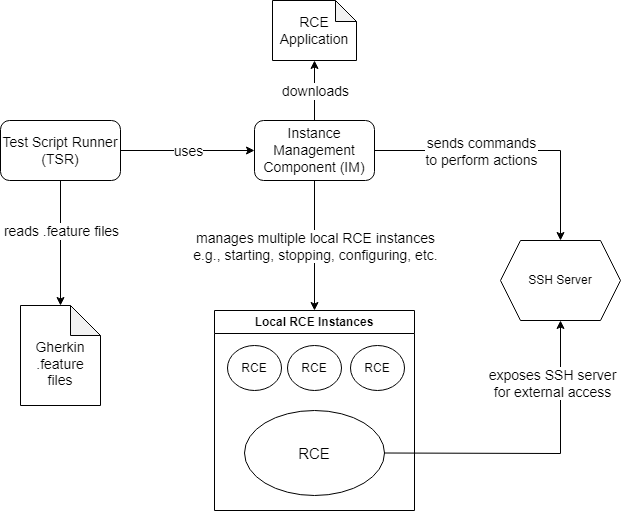
\includegraphics[scale=0.50]{files/figures/RCE-Setup.png}
    \caption{Illustration of the interplay between the Test Script Runner (TSR), Instance Management Component (IM), and RCE instances}
    \label{fig:rce-setup}
\end{figure}

Based on the illustrated RCE Setup in~\Cref{fig:rce-setup}, in which \ac{TSR} utilizes this \ac{SSH} connection for its communication to monitor and control local \ac{RCE} instances, we analyzed the source code and observed that, indeed, \ac{TSR} communicates over \ac{SSH} and extracts all necessary status information from the output of the \ac{SSH} session. In this context, the \ac{TSR} does not create or manage these \ac{SSH} connections itself; instead, this responsibility is delegated to the \ac{IM}. This means that the \ac{TSR} genuinely relies on the \ac{IM} for access and communication with \ac{RCE} instances. Consequently, theoretically transitioning from a local execution approach to a distributed, real-world, cloud-based scenario is straightforward with a simple adjustment of the \ac{IM}.

\subsubsection{Conclusion and Feedback}
In conclusion, RCE features a dedicated component, the \acf{TSR}, which acts as the interface between Gherkin and the execution of tests. It encapsulates all the relevant mappings and business logic required for the execution of tests written in Gherkin. Notably, the logic for initiating and controlling instances is abstracted through the \acf{IM}. \ac{TSR} relies on the \ac{IM} for managing \ac{SSH} connections, delegating responsibility for access and communication with RCE instances. The distribution of the application is facilitated by locally launching multiple RCE instances and controlling them via \ac{SSH}. This approach enables the simulation of a distributed system, providing a more realistic testing environment. It eliminates the need to configure and deploy RCE to an actual distributed system for testing, thus simplifying the local debugging of tests.

A drawback of this setup is that communication over the loopback device rarely exposes network-related error sources. Consequently, testing whether RCE can handle these errors correctly is a challenge. One significant reason for this limitation is that the loopback device provides a virtual network interface exclusively for local communication on the same machine. Therefore, it lacks the complexities and potential issues associated with actual network communication, such as latency, packet loss, and varying network conditions.


Therefore, it would be interesting to explore an alternative approach to simulate network errors, such as inducing latency, packet loss, or network congestion, within the test setup. Examples of such simulations could include introducing artificial delays in communication between \ac{RCE} instances or deliberately dropping packets to assess how \ac{RCE} handles such scenarios. Ideally, executing the tests in a distributed manner, involving individual \ac{RCE} instances in a cluster rather than launching them on a local machine, would provide a more realistic simulation. The abstraction of these tasks by the \ac{IM} makes this theoretically achievable with minimal dependencies due to the abstract implementation of the \ac{IM}. In~\Cref{sec:results}, we present a potential solution to introduce artificial network faults, even within the underlying local setup.

\subsection{Evaluating Fault Tolerance: Provoking Failures in \ac{RCE} Tests}
\label{subsec:fault-tolerance}
This section centers on the evaluation of fault awareness or tolerance within the current suite of \ac{BDD} tests in \ac{RCE}. Our motivation comes from the identification of specific waiting conditions, such as ensuring the successful launch of necessary RCE instances by the \ac{IM}, as mentioned earlier in~\Cref{subsec:PreparingRCETests}. The objective of our examination is to determine the resilience of these waiting conditions, scrutinizing their adaptability to varying system resources, and assessing whether they might contribute to test failures that surpass the predefined wait-for-seconds threshold, because of insufficient resources rather than faulty implementations. An illustrative example of these static waits is presented in~\Cref{lst:staticwait}.

\begin{listing}[!ht]
\caption{Waiting step in Gherkin Scenario}
\label{lst:staticwait}
\inputminted[linenos, xleftmargin=2em]{gherkin}{files/code/staticwait.feature}
\end{listing}

Now, consider the test step in line 4 and it's corresponding implementation, introduced in \Cref{lst:staticwait_impl}. 

\begin{listing}[!ht]
\caption{Step Definition for waiting step in Gherkin Scenario}
\label{lst:staticwait_impl}
\inputminted[linenos, xleftmargin=2em]{java}{files/code/staticwait_impl.java}
\end{listing}

In line 7 of the step definition, Java's \texttt{Thread.sleep}\footnote{\seqsplit{https://docs.oracle.com/en/java/javase/11/docs/api/java.base/java/lang/Thread.html}} method is used, that pauses the current thread for at least the specified number of seconds. Using static waits to ensure a desired system state may present challenges, as the predefined time duration might be insufficient and cannot adapt to the available resources in the testing environment. Specifically, the use of static waits can lead to test failures in scenarios where resource availability is limited and required processes cannot be completed within the allocated time. On the other hand, this method may introduce unnecessary delays in test execution when resources are highly efficient and capable of completing tasks more rapidly than expected.

To empirically assess the tolerance of static wait durations under constrained resource conditions, we implemented a controlled experimental setup using a \ac{VM}. The \ac{VM} was hosted on the following bare metal host system, as illustrated in~\Cref{lst:host-specs}:

\begin{listing}
\caption{Host System Specs}
\label{lst:host-specs}
\inputminted{text}{files/neofetch-host.txt}
\end{listing}

On this system, we set up an Ubuntu 22.04 LTS machine using KVM/QEMU, with the specifications outlined in~\Cref{lst:vm-specs}.
\begin{listing}
\caption{\acl{VM} Guest Specs}
\label{lst:vm-specs}
\inputminted{text}{files/neofetch-test-host.txt}
\end{listing}

To rule out the presence of faulty tests, we ensured that executing the tests on the system specified in~\Cref{lst:host-specs} led to successful outcomes. In the experimental arrangement in~\Cref{lst:vm-specs}, we intentionally restricted the available resources of the \ac{VM}, notably reducing the RAM to 8 GB and constraining the CPU cores to 2. This was done to emulate an environment characterized by resource insufficiency. By imposing these limitations, our objective was to induce a test failure linked to the static wait issue, utilizing the 5-second threshold depicted in~\Cref{lst:staticwait}. 

While executing all tests on the \ac{VM} system, we observed that despite the short duration of 5 seconds, all ``GIVEN`` clauses were successfully executed. However, a significant number of workflow tests (i.e., \texttt{Workflow05}), failed to complete successfully. Workflow tests denote operations that involve extensive calculations, and the limited number of CPU cores became evident in this context. Upon inspecting the log outputs of the failed tests, we also noted that although the last log output of the test should have been displayed, it was empty. This is likely due to the ongoing computation on the side of the executing \ac{RCE} instance, resulting in a delay in reporting errors or successful messages.

To further investigate the impact of these static waits, we conducted additional tests, including running cpuburn\footnote{https://patrickmn.com/projects/cpuburn/} (similar to Prime95) to simulate increased CPU utilization. Executing a burn test test on our VM, inducing 80\% CPU utilization, resulted in failures in the ``GIVEN`` clauses' waits. It is noteworthy that an 80\% utilization, though seemingly uncommon, could realistically occur in a CI/CD test system with simultaneous execution of multiple tests. Furthermore, the computational performance of these systems may be lower than in our scenario with a single core of the 7940HS, particularly in cloud instances where portions of the cores, i.e. $\frac{1}{8}$, can be allocated to \acp{VM}.

Furthermore, we conducted tests involving manual closure of \ac{RCE} instances instantiated by \ac{IM}. This action aimed to simulate a Java error or crash of \ac{RCE}. Instances terminated in this manner also led to failed tests and were essentially not detected by the \ac{IM}. While this is not inherently problematic, it would be desirable for the \ac{IM} to monitor \ac{RCE} processes through a watchdog and evaluate the shutdown condition accordingly.

\subsection{Code Review of \ac{RCE}'s Testing Setup}
\label{subsec:CodeReview}
To conclude our analysis, we reviewed the source code of both the \ac{TSR} and \ac{IM}. This step was intended to ensure the correctness of the implemented step definitions and their alignment with their intended functionality. It was essential to verify that the step definitions execute the actions as expected and, in the case of ``THEN`` conditions, evaluate them appropriately, avoiding scenarios where, for example, they consistently produce positive evaluations.

During our analysis, we observed that the structure and organization of individual components generally adhere to key code quality principles, such as maintainability, modularity, and reusability. This manifests itself in a clear separation of concerns, as exemplified by the arrangement of the \texttt{\seqsplit{de.rcenvironment.supplemental.testscriptrunner.scripts}} project. Within this project, the feature files describe high-level scenarios, effectively decoupling the overarching behavioral specifications from their underlying implementations, which are stored in the \texttt{\seqsplit{de.rcenvironment.supplemental.testscriptrunner}} project. 

This delineation between the descriptive feature files and the implementation-specific code aligns with best practices in software architecture, promoting clarity and modularity. The adherence to these paradigms is also reflected in the internal structure within each project, ensuring a swift and comprehensible grasp of the project's intricacies. Additionally, it is evident that the business logic is decoupled through interfaces and concrete implementations, allowing the underlying implementations to be dynamically switched if needed. This is particularly positive in the case of \ac{IM}, as described above, which facilitates a relatively straightforward transition from local to remote execution of \ac{RCE} instances. 

One notable observation related to the \ac{IM} was that the \texttt{\seqsplit{InstanceManagementService}} seemed quite tailored to the current structure for local tests, where individual \ac{RCE} instances are downloaded locally by the \ac{IM}. Certain methods, such as \texttt{\seqsplit{getInstallationsRootDir, getVersionOfInstallation}}, and \texttt{getDownloadsCacheDir}, might become obsolete in different configurations. These methods could potentially be implemented without functionality if, for example, the tests are executed on an existing remote cluster, etc. Therefore, this observation is not particularly problematic and serves as a mere observation rather than a significant critique.

However, our analysis identified specific instances that warrant review. Numerous step definitions rely on complex regex patterns, where simpler and more readable Cucumber Expressions could be employed. This is particularly evident in the mapping of test steps within feature files to intricate regular expressions in Cucumber Step Definition annotations (cf. \Cref{fig:cucumber-mapping}). Consequently, this introduces additional cognitive stress for developers, compromising the readability of the code. The resulting complexity poses challenges for immediate comprehensibility, potentially impeding the ease of future modifications and collaborations. Although not pervasive, these readability issues have significance and can potentially impact overall maintainability, especially in scenarios that lack a direct correspondence between the test steps and their definitions.
\section{Results}
\label{sec:results}
In this section, we present a concise summary of our findings derived from the thorough examination. Initially, we revisit our observations concerning the current setup of RCE, highlighting the identified issues and challenges in~\cref{sub:identified-problems}. Subsequently, we delve into the aspect of missing network fault tests, shedding light on the implications and gaps observed in this critical area of RCE's testing framework in~\cref{sub:lack-network-tests}. 

\subsection{Identified problems in RCE's Testing Setup}
\label{sub:identified-problems}
In this section, we will address identified problems in RCE's testing setup, structuring our discussion around three key points: the presence of static waits, the intricate use of complex regex patterns, and the lack of network tests simulating faults
.
\subsubsection{Static WAITs}
In numerous scenarios within \ac{RCE}'s testing setup, processes such as the execution of workflow” or ensuring a specific system state rely on static waits. Our analysis, particularly in~\cref{subsec:staticwaits}, highlighted the limitation of this approach, especially when the system environment requires more time than the predefined static wait duration. This mismatch can lead to unnecessary test failures. To address this, we recommend the adoption of dynamic waits or conditional waits where feasible. While dynamic waits with timeouts might be suitable in cases where checking for workflow completion is challenging, implementing these adaptive strategies enhances the resilience of tests to variable system conditions. Alternatively, the method of timeouts, already used in the Network Tests (e.g., "@Network02" with the "THEN"-clause "should be ready within 20 seconds"), can be applied. This approach employs periodic checks within a specified timeframe, serving as a timeout implementation that adapts to varying system conditions.


\subsubsection{Suboptimal Application of Regex in Cucumber Step Definitions}
\label{subsec:resultCucumber}

In~\cref{subsec:CodeReview}, we highlighted the challenges posed by the use of \ac{Regex} in Cucumber annotations, particularly concerning their impact on readability and simplicity. The intricate syntax of \ac{Regex}, while offering robust pattern-matching functionality, tends to result in annotations that are complex and challenging to interpret, especially for individuals lacking proficiency in \ac{Regex}. The introduction of Cucumber Expressions offers a solution to the identified issues, providing a simpler, more intuitive syntax that enhances readability and comprehensibility, thereby alleviating the cognitive stress while improving overall code maintainability. For an illustrative contrast between a step-definition annotation utilizing \ac{Regex} and one employing Cucumber Expressions, refer to~\cref{lst:simpleRegex}.

\begin{listing}[!ht]
\caption{simple \ac{Regex} annotation}
\label{lst:simpleRegex}
\inputminted{java}{files/code/simpleRegex.java}
\end{listing}

In this example, the ease of using Cucumber Expressions becomes evident. In contrast to the necessity for users to have a comprehensive understanding of capturing groups, character classes, negation, and quantifiers in order to decipher this particular \ac{Regex}, Cucumber Expressions and their intuitive placeholders (e.g., "\{string\}, \{int\}, \{float\}, etc.)", offer a starkly different user experience when capturing primitive data types.

While Cucumber Expressions offer improved readability and ease of use, it is important to acknowledge that they do not possess the same level of expressive power as \ac{Regex}. This distinction introduces a trade-off between simplicity and flexibility, that will be further discussed in~\cref{sec:discussion}.


\subsubsection{Lack of Genuine Network Tests Incorporating Network Faults}
\label{sub:lack-network-tests}

In the current test setup, the network aspect of the application is examined on the localhost by initiating multiple local instances. However, this approach might overlook critical real-world circumstances present in an actual distributed environment. As the current setup lacks the capability to test the application's behavior under conditions like packet loss or connection timeouts, it becomes imperative to implement additional tests focusing on these specific failures. Since there is no built-in method in Java to simulate such failures, external tools like WinDivert or Chaos Mesh can be utilized.

WinDivert, designed for Windows, can intercept network traffic at the kernel level, enabling the introduction of network faults. Although it has Java bindings and can be seamlessly integrated into the existing suite, creating specific network faults would require manual intervention, as the library primarily offers basic methods for monitoring, modifying, or dropping packages. On the other hand, tools like Chaos Mesh, built upon \ac{K8S}, can independently generate various network faults. However, they require the execution of tests within a \ac{K8S} cluster. This, in turn, requires the setup and configuration of either a local \ac{K8S} cluster (e.g., minikube) or the use of a remotely hosted cluster, thus adding to the initial setup complexity of the \ac{RCE} development process.
\section{Discussion}
In this section, we delve into a nuanced discussion regarding the strategic use of Cucumber Expressions as opposed to regular expressions (\ac{Regex}). In~\cref{subsec:expression-strategies} we will explore scenarios where the expressive power of \ac{Regex} may not be a limiting factor, making Cucumber Expressions a favorable choice. Additionally, in~\cref{subsec:network-fault-wdiviert-chaos-mesh}, we will scrutinize situations where the decision to use either WinDivert or Chaos Mesh for network fault testing depends on specific requirements and operating system considerations.

\subsection{Expression Strategies: Navigating the Choice Between \ac{Regex} and Cucumber Expressions}
\label{subsec:expression-strategies}

As discussed in~\cref{subsec:resultCucumber}, Cucumber Expressions offer several advantages in terms of their user-friendliness, as they are designed to be more intuitive and straightforward, making them an excellent choice for common scenarios where patterns are relatively simple and direct. However, their simplicity comes at the cost of the extensive pattern-matching capabilities inherent to \ac{Regex}, that allow intricate and nuanced string manipulation, capable of handling a wide range of complex scenarios and edge cases with precision. 

\begin{listing}[!ht]
\caption{Code snippet showing a complex \ac{Regex} annotation}
\label{lst:complexRegex}
\inputminted{java}{files/code/complexRegex.java}
\end{listing}

In scenarios such as those illustrated in~\cref{lst:complexRegex}, Cucumber Expressions prove inadequate for replacing a regular expression, particularly when the latter includes a nested optional statement. This limitation arises from the fact that Cucumber Expressions do not support nested optional statements, rendering them unsuitable for scenarios where such complexity is present in the regular expression. In addition, there are instances, such as with the regular expression \verb|^[Ww]aiting for (\\d+) second[s]?$| and its corresponding Cucumber expression \verb|Waiting/waiting for {int} second(s)|. In these cases, a valid argument can be made that these expressions are equally effective, and there is no clear winner between them.

In summary, Cucumber Expressions offer a more user-friendly approach, facilitating a clearer and more straightforward composition of test cases, particularly advantageous for individuals with limited expertise with Regex. When intricate pattern-matching capabilities inherent in Regex are deemed non-essential, the adoption of Cucumber Expressions can significantly enhance the efficiency and collaboration within the development process. This choice aligns with the overarching objectives of simplicity and clarity in the practices of test automation.

Therefore, the RCE developers are urged to evaluate the specific requirements of their context when confronted with the decision between the two approaches. This involves carefully considering the trade-off between the benefits of simplicity and the necessity for comprehensive pattern-matching capabilities. As a general guideline, it is advisable to employ Cucumber Expressions whenever possible, especially in cases, e.g.,~\cref{lst:simpleRegex}, where regular expressions solely aim to capture primitive input types and do not involve intricate conditional logic.

\subsection{Network Fault Simulation Tools: Choosing Between WinDivert and Chaos Mesh}
\label{subsec:network-fault-wdiviert-chaos-mesh}
Simulating network faults is a crucial aspect of testing to ensure the robustness and reliability of distributed systems. In this section, we compare two tools, WinDivert and Chaos Mesh, each offering distinct advantages and drawbacks.

\subsubsection{WinDivert:}
At first glance, WinDivert appears to be a straightforward and practical solution for simulating network faults. Its simplicity and compatibility with Java make it an attractive option, especially for local tests through the \ac{IM} implementation. However, upon closer inspection, WinDivert reveals its more primitive nature, necessitating the manual implementation of network faults and their associated logic. While suitable for basic scenarios, this approach becomes less suitable for a more comprehensive and dynamically modeled error simulation, additionally shifting the responsibility of correctly implementing network failures to the development team.

\subsubsection{Chaos Mesh:}
Chaos Mesh, built on Kubernetes, provides a more advanced and comprehensive solution for simulating network faults. Its capabilities extend beyond simple network simulations, encompassing a variety of faults, including those related to the Java Virtual Machine (JVM), the kernel, memory, disk bandwidth, and more. Although requiring an initial shift of the testing environment to Kubernetes, it aligns with a long-term testing strategy that requires a diverse range of error scenarios.

\subsubsection{Recommendation:}
Considering these factors, we recommend a hybrid testing approach that leverages the strengths of both WinDivert and Chaos Mesh. For debugging purposes and local tests with the existing \ac{IM}, WinDivert offers simplicity and user-friendliness, allowing developers to quickly identify and address specific network faults. This approach is particularly valuable for scenarios where debugging within a Kubernetes environment might be challenging, and for scenarios that do not require extensive fault simulations.

On the other hand, we advocate for the extensive and comprehensive simulation of network faults using Chaos Mesh within a Kubernetes cluster. This strategy ensures a broader coverage of network-related issues and aligns with a long-term testing approach that encompasses a variety of faults beyond simple network simulations.

In summary, the proposed approach combines WinDivert for initial debugging and local tests with the use of Chaos Mesh for more sophisticated and comprehensive simulation of network faults within a Kubernetes environment. This hybrid methodology combines the practical benefits of both tools, facilitating efficient debugging and comprehensive error testing, thus offering a balanced testing strategy.
\section{Conclusion}
\label{sec:conclusion}
In the course of this paper, we have explored the intricacies of the existing RCE testing setup. Our investigation revealed that \acf{BDD} tests are conducted using the Cucumber library and are orchestrated through a component known as \acf{TSR}, which relies on the \acf{IM} to simulate a distributed system on a local machine, as depicted in~\Cref{fig:rce-setup}. This is achieved by launching multiple RCE instances locally and facilitate communication via the loopback device. 

An in-depth examination of the codebase revealed notable issues, particularly the reliance on static waits and the utilization of intricate regex patterns, as well as the absence of genuine network tests that incorporate common network faults. We have elucidated the potential ramifications of these issues and proposed viable solutions, such as the adoption of dynamic waits and conditional waits for improved adaptability, and the introduction of Cucumber expressions to enhance readability and comprehensibility. Moreover, we proposed the integration of tools like Chaos Mesh, a solution capable of simulating various network faults and resource throttling within a \acf{K8S} environment, to target the missing network failure test. This recommendation positions Chaos Mesh as a versatile tool that not only addresses current requirements, but also offers scalability for potential future testing needs. Alternatively, for scenarios where Windows is the predominant operating system, WinDivert emerges as a feasible solution. Its simplicity and Java compatibility make it an attractive option, though it is limited to Windows environments. 

In conclusion, our comprehensive analysis provides valuable insights into the strengths and areas for enhancement within the RCE testing setup. We believe that addressing these identified issues, could improve the reliability and effectiveness of the testing infrastructure, while also aligning it more closely with real-world testing scenarios. Despite the challenges addressed, the modular and decoupled design of the \ac{IM} and \ac{TSR} components emerged as commendable strengths, improving maintainability and flexibility in the testing architecture.


%
% ---- Bibliography ----
%
% BibTeX users should specify bibliography style 'splncs04'.
% References will then be sorted and formatted in the correct style.
%
\bibliographystyle{splncs04}
\bibliography{references}
\end{document}
